\documentclass{article}

% ML x OR @ NeurIPS 2026: 4-page main body, NeurIPS conference format,
% non-anonymous ([final]), unlimited references + appendix.
% Swap neurips_2025.sty for the official neurips_2026.sty when released.
\usepackage[final]{neurips_2025}

\usepackage[utf8]{inputenc}
\usepackage[T1]{fontenc}
\usepackage{hyperref}
\usepackage{url}
\usepackage{booktabs}
\usepackage{amsfonts}
\usepackage{nicefrac}
\usepackage{microtype}
\usepackage{graphicx}
\usepackage{xcolor}
\usepackage{macros}   % shared with the derivation folder: theorem envs, \eps, \gpo, ...

\graphicspath{{figures/}}

% Workshop footer (the sty hardcodes the main-conference notice)
\makeatletter
\renewcommand{\@noticestring}{%
  Second Workshop on ML$\times$OR at NeurIPS 2026, Atlanta, GA.}
\makeatother

\title{PRICE: Minimax Estimation--Regret Tradeoffs and\\ Certified Exploration in Performative Prediction}

\author{%
  Shriraghav Ashok\thanks{Equal contribution.} \\
  \texttt{shriraghav.a524@gmail.com}
  \And
  Vignesh Nagarajan\footnotemark[1] \\
  \texttt{vignesh.nagarajan@[institution].edu}
}

\begin{document}

\maketitle

\begin{abstract}
A decision-maker whose deployed policy reshapes its own data distribution must pay, in its own objective, to learn how it moves the world. We price that self-knowledge exactly. In a structural performative market (a market maker whose quoted spread summons adverse flow), we prove a conservation law: along any stationary exploration policy, the variance of the response-slope estimate times the cumulative performative regret equals $\tfrac{1}{2}\gpo\sigma^2$ --- an invariant of the environment, not of the policy. We complement the identity with minimax lower bounds (exact for deviation budgets; sharp-constant for value budgets over two-point priors, with adversarial numerics showing the floor survives full knowledge of the response family), an optimal-design theory (shape exploration as $\Gpo^{-1/2}$; isotropic exploration overpays by an explicit dispersion factor), and a deployable agent, SafeD-PerfGD, that corrects its gradient only when an anytime confidence sequence certifies, through a perturbed-modulus lemma, that the correction cannot destabilize its own retraining loop. Every closed form is verified in a live deploy--observe--fit--correct pipeline (36 preregistered measured-vs-predicted checks, 0 failures), transplanted exactly to a second economy, and instantiated on a real-data corporate-bond calibration that reproduces its published source 10/10 cells. Code, derivations, and all checks: \url{https://github.com/[repo]/price}.
\end{abstract}

\section{Introduction}
\label{sec:intro}

When a deployed model changes the distribution it is trained on, retraining becomes a fixed-point iteration: performative prediction \citep{perdomo2020performative} shows repeated risk minimization converges iff the distribution's sensitivity $\eps$ is small against the loss curvature $\gamma$ ($m = \eps\beta/\gamma < 1$), and converges to a \emph{performatively stable} point that is not the \emph{performative optimum}. Algorithms that close this gap --- performative gradient descent and its descendants \citep{izzo2021learn,miller2021outside} --- all consume an estimate of the distribution's response $dD/d\theta$, obtained by perturbing deployments. The literature treats the accuracy of that estimate as an assumption and the perturbations as free. Neither is: the perturbations are deployments of a real decision variable, and their cost lands in the decision-maker's own objective. \emph{What does it cost to learn your own influence?} This paper answers with an identity, a floor, a design rule, and an agent.

\textbf{Contributions.}
\begin{enumerate}\itemsep1pt\topsep2pt\parsep0pt
\item \textbf{A conservation law (\S\ref{sec:price}).} Along any stationary exploration policy, $\Var(\hat\eps)\times C_T = \tfrac{1}{2}\gpo\sigma^2$: slope uncertainty times cumulative performative regret is a policy-independent invariant (Theorem~\ref{thm:exchange}). The anchoring is delicate: the same product anchored at the performative optimum is \emph{false}, inflated by a factor we verify.
\item \textbf{Minimax floors (\S\ref{sec:price}).} No non-anticipating policy beats the floor: exactly under deviation budgets; with sharp constant over two-point priors, and within a factor $\le 13.5$ in general, under value budgets (Theorem~\ref{thm:devbudget}). Adversarial numerics show the floor is \emph{structure-proof} (best family-knowing design: $1.005\times$ the floor) and map its exact boundary: curvature uncertainty protects it.
\item \textbf{Optimal exploration design (\S\ref{sec:design}).} Under a budget priced by the decision-maker's own curvature, the optimal exploration covariance is $\Gpo^{-1/2}$-shaped; isotropic exploration overpays by the dispersion factor $F = d\,\tr\Gamma/(\tr\Gamma^{1/2})^2$ --- a quotable inversion of ``naive exploration is optimal'' for LQR \citep{simchowitz2020naive}. A support-degeneracy theorem and a misspecification crossover complete the design picture.
\item \textbf{A certified agent (\S\ref{sec:design}--\ref{sec:experiments}).} SafeD-PerfGD explores on a D-optimal support, fits an anchored response family with an anytime confidence sequence, and applies the performative correction only when a perturbed-modulus certificate guarantees closed-loop stability --- otherwise it freezes the correction while the provably-stable blind step keeps running. It reaches the performative optimum where blind retraining stalls; no published baseline Pareto-dominates it on (final error, regret).
\end{enumerate}

\textbf{Positioning.} \citet{jagadeesan2022regret} bound the regret of \emph{finding} the performative optimum; we price \emph{knowing your own feedback} --- lower bounds and an invariance identity where they give algorithmic upper bounds, with no retraining loop, stability constraint, or design shaping in their model. \citet{lin2024plugin} show misspecified structural models still help performative optimization; our crossover theorem sharpens that message into a budget-explicit rule. In operations research, incomplete learning under myopic pricing is classical \citep{rothschild1974two,harrison2012bayesian,keskin2014dynamic,broder2012dynamic,denboer2015dynamic}, and \citet{lai1979adaptive}'s adaptive designs are \emph{points on} our frontier --- but the frontier itself, its minimax floor over adaptive policies, and the performative loop generating it do not appear: the demand curve is exogenous throughout. From control we inherit dual control \citep{feldbaum1960dual} and least-costly identification \citep{bombois2006least} --- here the plant is a retraining learner, the budget the optimizer's own objective, the constraint loop contraction; task-optimal design \citep{wagenmaker2021task,dean2020sample} supplies machinery the classical canon \citep{kiefer1960equivalence,pukelsheim2006optimal} never prices in the experimenter's objective. Lower bounds are van Trees arguments \citep{gill1995applications}; a claim-by-claim novelty crosswalk ships with the repository.

\section{Model}
\label{sec:model}

A dealer quotes half-spread $h$. Benign flow arrives at rate $U(h) = A e^{-kh}$; informed (toxic) flow at rate $\tau(h) = C_0 + C_1 e^{-c h}$: tighter quotes summon more toxic flow. Profit at frozen toxic level $T$ is $J(h;T) = h\,U(h) + (h - \psi)\,T - w (h - h_{\mathrm{ref}})^2$ ($\psi$: adverse severity; $w$: quoting-cost convexity); the \emph{performative value} is $\Phi(h) = J(h,\tau(h))$. Write $\eps(h) = -\tau'(h)$ for the response slope (the scalar $dD/d\theta$), $\gamma = -\partial^2_h J$, and $\gpo = -\Phi'' = \gamma + \eps\,(2 + c\psi - ch)$. Blind retraining (RRM) is the cobweb $h_{t+1} = \mathrm{BR}(\tau(h_t))$, a contraction iff the modulus $m = \eps/\gamma < 1$ \citep{perdomo2020performative}; it converges to the stable point $\hsp$, while the optimum $\hpo = \arg\max\Phi$ sits at a wider spread --- the echo-chamber gap \citep{miller2021outside}. Deployments return noisy flow $y_t = \tau(h_t) + \sigma\xi_t$ (A2). The estimand is $\eps$ at the operating point; exploration deviations $\dev_t = h_t - \hstar$ are priced by the \emph{incremental} cost $C_T = \sum_{t \le T} \E[\Phi(\hstar) - \Phi(h_t)]$, anchored at the certainty-equivalent operating point $\hstar$ (A1: local quadratic scope; A3: stationary exploration scale). Results are stated for this scalar family and, where flagged, its $d$-dimensional and linear-quadratic instances; full statements and proofs are in Appendices~\ref{app:theorems}--\ref{app:proofs}.

\section{The price of self-knowledge}
\label{sec:price}

\textbf{Free data saturates.} Without deliberate exploration the retraining trajectory's identifying energy is finite: for deployment error $d_0$ and modulus $m$ it is capped at $d_0^2/(1-m^2)$ (T1; matrix version by a Lyapunov identity). A corollary was discovered by a failed prediction (\S\ref{sec:experiments}): retraining on \emph{noisy} observations converts observation noise to deployment noise with gain $1/\gamma$, adding a stationary excitation floor $(\sigma/\gamma)^2/(1-m^2)$ per step; both closed forms verify. The stabler the loop, the less it reveals: \emph{safety implies blindness} --- the performative sharpening of incomplete learning under myopic policies \citep{keskin2014dynamic,harrison2012bayesian}, where the stall comes from optimization converging rather than from the feedback strength itself.

\textbf{The exchange rate.} Deliberate exploration buys information at an exact, policy-independent price.

\begin{theorem}[Exchange rate; T2]
\label{thm:exchange}
Under A1--A3, for the OLS slope estimator on any stationary exploration policy with deviations $\{\dev_t\}$,
\[
\Var(\hat\eps)\;\times\;C_T \;=\; \tfrac{1}{2}\,\gpo\,\sigma^2\;\big(1 + o(1)\big),
\]
independent of the exploration amplitude, shape, and schedule, and of the modulus $m$.
\end{theorem}

The mechanism is cancellation: information scales as design energy $S_T=\sum_t(\dev_t-\bar \dev)^2$, cost as $\tfrac{1}{2}\gpo\sum_t \dev_t^2$; for mean-centered exploration these are the same sum. \emph{Anchoring}: the same product anchored at $\hpo$ is false --- inflated by an explicit factor, falsified numerically before the incremental version was proved; the invariant prices \emph{exploration}, not \emph{suboptimality}. \emph{Invariance}: \citet{lai1979adaptive} exhibit schemes with $O(\log n)$ cost and efficient estimation --- consistent points on this frontier --- but the identity says \emph{every} stationary policy lies on it. A corollary prices the echo chamber: closing $\hsp - \hpo$ pays iff the horizon exceeds an explicit break-even (Appendix) --- rational incomplete learning \citep{rothschild1974two,easley1988controlling,aghion1991optimal} in closed form.

\textbf{Minimax floors.} The identity is for OLS-on-stationary policies; the floors are for everyone.

\begin{theorem}[Minimax floors; T3--T4]
\label{thm:devbudget}
(i) Over all non-anticipating (possibly randomized, adaptive) policies with expected design energy $\E S_T \le B$: $\inf \sup \Var(\hat\eps) \ge \sigma^2/B$, hence the product floor holds exactly. (ii)~Under a budget on realized performative cost with certainty-equivalent anchoring, the floor $\tfrac{1}{2}\gpo\sigma^2(1-o(1))$ holds with sharp constant over two-point symmetric priors (correction rate $T^{-1/2}$), and within constant factor ($\ge \gpo\sigma^2/27$, Le~Cam) over general priors.
\end{theorem}

Closing the general-prior sharp constant is open; we attacked its premise adversarially. Minimizing the Cram\'er--Rao product over all designs \emph{within the known three-parameter family} yields $1.005\times$ the floor under both cost models, the optimizer collapsing back to the symmetric two-point configuration --- consistent with the least-favorable-two-point reduction the proof strategy requires --- while tight-side probing (sensitivity $e^{-ch}$) is monotonically \emph{worse} (ratio $5.7 \to 41$): remote information must be pulled back through $\hat c$, and extrapolation variance dominates the sensitivity gain. The boundary is exact: with $c$ known a priori the floor breaks (ratio $\to 0.05$). \emph{The floor is an ignorance-of-curvature phenomenon} --- the correct scope for the general theorem.

\begin{figure}[t]
\centering
\begin{minipage}{0.34\textwidth}
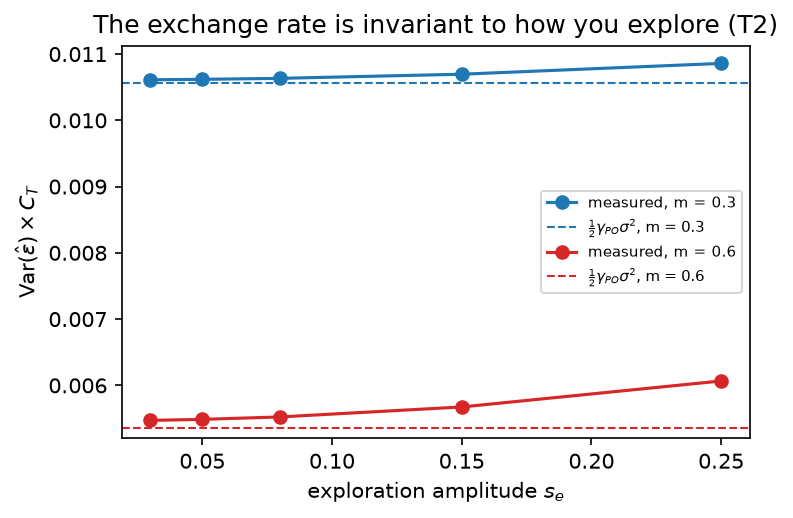
\includegraphics[width=\textwidth]{fig1_exchange_rate.png}
\end{minipage}\hfill
\begin{minipage}{0.34\textwidth}
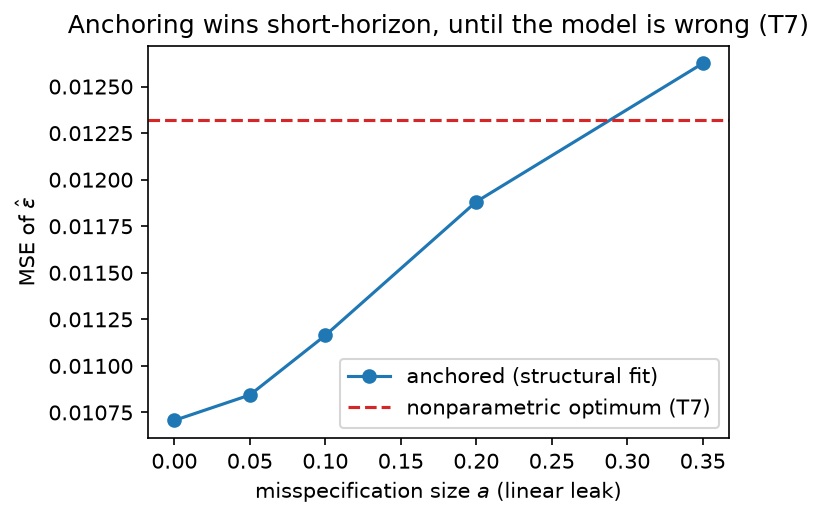
\includegraphics[width=\textwidth]{fig4_crossover.png}
\end{minipage}
\caption{\textbf{Left:} measured $\Var(\hat\eps)\times C_T$ vs exploration amplitude, two moduli: flat on the invariant (dashed), with the small large-amplitude drift the local scope predicts. \textbf{Right:} the anchoring crossover (T7): structure beats nonparametrics until misspecification crosses the closed-form threshold.}
\label{fig:exchange}
\end{figure}

\section{Optimal design and certified correction}
\label{sec:design}

\textbf{Shape (T5).} In $d$ dimensions with curvature $\Gpo \succ 0$ pricing the budget $\tfrac12\E[u^\top\Gpo u]$, the A-optimal exploration second moment is $M^* \propto \Gpo^{-1/2}$: explore \emph{where your objective is flat}. Isotropic exploration overpays by exactly the dispersion factor $F = d\,\tr\Gpo/(\tr\Gpo^{1/2})^2 \in [1, d]$: naive exploration, optimal for LQR \citep{simchowitz2020naive}, is suboptimal here by precisely $F$ --- task-optimal design \citep{wagenmaker2021task} where the task is the learner's own objective. \textbf{Support (T6).} The exponential family is Chebyshev-degenerate on thin designs: fewer than three support points (or vanishing spread, or collinear probe schedules) cannot identify $(C_0, C_1, c)$ --- a cliff we later hit twice in the wild (\S\ref{sec:experiments}). \textbf{Anchor (T7).} With budget $B$ and horizon $T$, fitting the structural family beats nonparametric slope estimation iff the misspecification at the operating point is below $|\tau'''|B/(3\gpo T)$ --- \citet{lin2024plugin}'s qualitative message sharpened to a decision rule priced in the exploration budget itself.

\textbf{The agent.} SafeD-PerfGD composes the three results per deployment round: (i) \emph{explore} on the D-optimal three-point support re-centered at the operating point, trust-region clipped; (ii) \emph{fit} $(C_0, C_1, c)$ by profile least squares with an anytime self-normalized confidence width $\mathrm{ci}_t$ for $\hat\eps$; (iii) \emph{gate}: apply the performative correction $-(h-\psi)\hat\eps$ with Newton scaling $\eta = 1/\hat\gamma_{\mathrm{PO}}$ only if $\eta \cdot \mathrm{ci}_t \cdot L_{\mathrm{fam}} \le \text{margin}$, where the perturbed-modulus lemma (L4) with the family's own Lipschitz constant $L_{\mathrm{fam}} = 1 + \hat c\,|h - \psi|$ converts estimation error into a certified bound on the closed-loop modulus; (iv) otherwise \emph{freeze} the correction --- the blind step, provably stable at $m<1$, keeps running under the current fit. The freeze is derived, not tuned: it is what the certificate licenses. Safety holds throughout on the confidence-sequence event, and certification is not free --- the gate opens only after enough design energy accumulates, which by Theorem~\ref{thm:exchange} \emph{is} a regret payment (Figure~\ref{fig:gate}).

\begin{figure}[t]
\centering
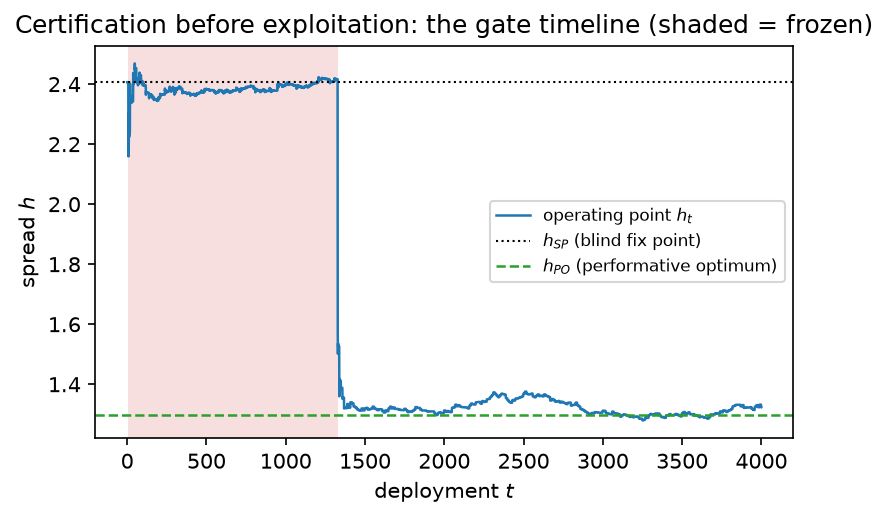
\includegraphics[width=0.41\textwidth]{fig3_certification.png}
\caption{Certification before exploitation: the agent holds near the blind fixed point $\hsp$ for ${\sim}1{,}300$ deployments while the confidence sequence tightens (shaded: frozen), then the certificate clears and it steps to $\hpo$. Certification time is the exchange rate at work.}
\label{fig:gate}
\end{figure}

\section{Verified results}
\label{sec:experiments}

Every claim above is a preregistered row in a measured-vs-predicted harness run against a live deploy--observe--fit--correct pipeline: \textbf{36 rows, 0 failures} (35 pass, one deliberately out-of-scope drift cell measured, not excused). Ten pivots were forced by measurement and recorded in code; three became results (the feedback floor, the false $\hpo$-anchored identity, the structure-proofness scope). Headline rows (Table~\ref{tab:results}, Appendix~\ref{app:table}): the exchange rate within $1$--$6\%$ across four (modulus, amplitude) cells; the feedback floor within $1$--$7\%$; the isotropic/A-optimal ratio matching $F$ ($1.529$ vs $1.506$); the D-design identifying $c$ where narrow jitter cannot ($7.8\times$, Fisher-consistent).



\textbf{Baselines.} Against finite-difference PerfGD \citep{izzo2021learn}, zeroth-order P\&L optimization, a performative-confidence-bounds explorer \citep{jagadeesan2022regret}, and blind RRM on identical environments, none Pareto-dominates SafeD-PerfGD on (final error, regret); the unsafe gradient baseline pays $>5\times$ its regret. Deliberately reported: the UCB explorer attains \emph{lower raw regret} --- certification is a real cost, and its visibility is the thesis. \textbf{Second economy.} Transplanted unchanged to LQ performative pricing (deployed price anchors demand), the exchange rate is exact in all four cells --- A1 is global in an LQ model, so the drift vanishes as predicted --- and the agent reaches the pricing optimum ($12.58$ vs.\ $12.5$) once its deterministic probe schedule was randomized: alternating probes make price and lag collinear, a T6 degeneracy met in the wild. \textbf{Real data.} On a public-data corporate-bond calibration (10 rating $\times$ regime cells), the port reproduces its published source \textbf{10/10} cells ($h^*$, $\eps^* = \gamma$, $m$ within $0.5$--$5\%$), then extends it: $\gpo$ spans $510.6$ to $2.3$; echo-chamber gaps are $2$--$4\%$ of the anchor spread; and the shaping dispersion is $F = 1.63$ \emph{across} the portfolio against $1.002$ within one book --- the gain lives across ratings and regimes, where a desk actually allocates exploration.

\paragraph{Limitations and outlook.}\label{sec:limits} The identity is local (A1): wide-side probing undercuts it polynomially at finite amplitude and the saturating cell drifts $+16\%$ --- the $o(1)$-amplitude qualifier is load-bearing. The value-budget sharp constant beyond two-point priors is numerically supported, not proved; the register's open problems are the workshop-to-journal delta. At matched transit energy, full-support jitter identifies on par with the design, whose advantage is small-amplitude and allocational. Calibrated moduli are deeply stable and the toxic channel structurally scaled: the real-data leg validates machinery, not effect size. The framework also prices what a deployed generative system pays to learn its own influence on data it retrains on --- certified correction as a template for agentic closed-loop deployment.

\bibliographystyle{plainnat}
\bibliography{references}

\clearpage
\appendix

\section{Theorem statements (register copy)}
\label{app:theorems}
\input{theorems_body}

\section{Proofs}
\label{app:proofs}

Throughout, the local model of Assumptions A1--A6, per the derivation
folder's notation-and-assumptions register:
\textbf{A1} (local quadratic scope): $\Phi$ is $C^3$ and strongly concave
on the operating interval, expansions taken at $\hstar$ with third-order
remainder bounded by $L_3 = \sup|\Phi'''|$;
\textbf{A2} (exploration class): all policies are non-anticipating, with
A2-sym additionally requiring $\E[u_t \mid \mathcal{F}_t] = 0$ and
A2-adaptive unrestricted, costs measured from the certainty-equivalent
anchor;
\textbf{A3} (noise exogeneity): $\zeta_t$ i.i.d., mean zero, variance
$\sigma^2$, independent of $\mathcal{F}_t$;
\textbf{A4} (trust region): $|\dev_t| \le r$ pathwise;
\textbf{A5} (stationary scale): $S_T = \Theta(T)$;
\textbf{A6} (stable base loop): $m < 1$, equivalently $\rho(M) < 1$.
The local dynamics are $\dev_{t+1} = -m\,\dev_t + u_t$ with
$\dev_t = h_t - \hstar$ ($\hstar$ the certainty-equivalent operating
point, equal to $\hsp$ for the blind loop), observations
$\tau_t = \tau(\hstar) - \eps\,\dev_t + \zeta_t$, and $\Phi$ satisfying
$\Phi'(\hstar) = \delta_0 \neq 0$ and $-\Phi'' = \gpo$ at the operating
point.

\subsection*{A. Cost equivalence and its fluctuations}

\begin{proof}[Proof of Lemma L1 (cost equivalence)]
Taylor's theorem with Lagrange remainder gives, for each $t$,
\[
\Phi(\hstar) - \Phi(h_t)
 = -\delta_0\,\dev_t + \tfrac{1}{2}\gpo\,\dev_t^2 + r_t,
 \qquad |r_t| \le \tfrac{L_3}{6}\,|\dev_t|^3,
\]
with $L_3 = \sup |\Phi'''|$ on the operating interval. Summing over
$t \le T$ and taking expectations, it remains to show
$\E[\sum_t \dev_t] = 0$ under A2-sym. The recursion gives
$\E[\dev_{t+1} \mid \mathcal{F}_t] = -m\,\dev_t + \E[u_t \mid \mathcal{F}_t]
= -m\,\dev_t$, so $\E[\dev_{t+1}] = -m\,\E[\dev_t]$ by the tower property,
and $\E[\dev_t] = (-m)^t\,\E[\dev_0] = 0$ when the loop starts at the
operating point or in the stationary regime. The quadratic term contributes
$\tfrac{1}{2}\gpo\,\E[\sum_t \dev_t^2]$, which is the claim.

For the variance decomposition, write the realized cost (net of the cubic
remainder) as $C = -\delta_0 X + \tfrac{1}{2}\gpo Y$ with
$X = \sum_t \dev_t$, $Y = \sum_t \dev_t^2$. Then
$\Var(C) = \delta_0^2 \Var(X) + \tfrac{\gpo^2}{4}\Var(Y)
- \delta_0\gpo\,\Cov(X, Y)$. Under Gaussian innovations the vector
$(\dev_1,\dots,\dev_T)$ is jointly Gaussian with mean zero, and every third
moment of a zero-mean Gaussian vector vanishes; since
$\Cov(X,Y) = \sum_{t,s}\E[\dev_t\,\dev_s^2]$ is a sum of third moments, it is
zero. (For non-Gaussian symmetric innovations the same conclusion follows
from the sign symmetry $\dev \mapsto -\dev$ of the stationary law.)
Verified: V0.1--V0.3, including the necessity check that an asymmetric rule
breaks the expectation identity by exactly $-\delta_0\,\E[\sum_t \dev_t]$.
\end{proof}

\subsection*{B. Saturation}

\begin{proof}[Proof of Theorem T1 (information saturation)]
Let $\rho(M) < 1$ and define $P = \sum_{t\ge 0} (M^\top)^t M^t$. The series
converges absolutely: by Gelfand's formula $\|M^t\| \le C\,\rho_0^t$ for any
$\rho(M) < \rho_0 < 1$ and some $C$, so the terms are dominated by
$C^2\rho_0^{2t}$. Termwise,
$M^\top P M = \sum_{t \ge 0} (M^\top)^{t+1}M^{t+1} = P - I$, so $P$ solves
the discrete Lyapunov equation, and if $Q$ is any other solution then
$P - Q = M^\top (P-Q) M = (M^\top)^k (P-Q) M^k \to 0$, giving uniqueness.
The energy identity is immediate:
$\sum_{t\ge 0} \|M^t \dev_0\|^2 = \dev_0^\top \big(\sum_t (M^\top)^t M^t\big)
\dev_0 = \dev_0^\top P\,\dev_0$. The directional version replaces $I$ by
$uu^\top$: $P_u = \sum_t (M^\top)^t uu^\top M^t$ solves
$P_u = uu^\top + M^\top P_u M$ and
$\sum_t (u^\top M^t \dev_0)^2 = \dev_0^\top P_u\,\dev_0$.

For the information claim: under A3 the log-likelihood of the observations
along the noiseless trajectory has Fisher information for the response
component along $u$ equal to $\sigma^{-2}\sum_t (u^\top \dev_t)^2 =
\sigma^{-2}\,\dev_0^\top P_u \dev_0$, which is finite and independent of the
horizon; the Cram\'er--Rao bound gives the stated variance floor for
unbiased estimators (the biased/minimax version is Theorem T3's van Trees
argument). Verified: V1.1, V1.2, V1.4.
\end{proof}

\begin{proof}[Proof of Corollary C1.1 (safety implies blindness)]
In the scalar case $P = \sum_t m^{2t} = (1-m^2)^{-1}$, so the cap
$(h_0-\hstar)^2/(1-m^2)$ has derivative in $m$ equal to
$2m\,(h_0-\hstar)^2/(1-m^2)^2 > 0$ for $m \in (0,1)$: strictly increasing.
\end{proof}

\begin{proof}[Proof of Corollary C1.2 (design degeneracy)]
For $m < 1$, $\dev_t = (-m)^t \dev_0$, so for every $\epsilon > 0$ all but
$\lceil \log(|\dev_0|/\epsilon)/\log(1/m)\rceil$ of the points lie in
$[-\epsilon, \epsilon]$: the empirical design measure converges weakly to
$\delta_0$. At $m = 1$, $\dev_t = (-1)^t \dev_0$ and the design measure is
$\tfrac{1}{2}(\delta_{+\dev_0} + \delta_{-\dev_0})$ exactly. In both cases
the limiting design has at most two support points; combined with Theorem
T6, the per-observation Fisher matrix of the three-parameter structural
family is asymptotically singular along the trajectory.
\end{proof}

\begin{proof}[Proof of Remark R1 (non-normal transient information)]
The identity $E(\dev_0) = \dev_0^\top P\,\dev_0$ of T1 holds for any stable
$M$, normal or not. If $M = V\Lambda V^{-1}$ is diagonalizable,
$\|M^t\| \le \kappa(V)\,\rho(M)^t$ gives
$\|P\| \le \kappa(V)^2/(1-\rho(M)^2)$. The bound is attained in order by the
Jordan-type family $M = \begin{pmatrix} m & a \\ 0 & m\end{pmatrix}$ with
$\dev_0 = e_2$: $M^t e_2 = (t\,a\,m^{t-1},\; m^t)^\top$, so
\[
E(e_2) = a^2 \sum_{t\ge 1} t^2 m^{2t-2} + \sum_{t \ge 0} m^{2t}
 = a^2\,\frac{1+m^2}{(1-m^2)^3} + \frac{1}{1-m^2},
\]
using $\sum_{t\ge1} t^2 x^{t-1} = (1+x)/(1-x)^3$ at $x = m^2$: the energy
grows as $a^2$, without bound, at fixed spectral radius. Verified: V1.3
(the exact value matches the Lyapunov solve; $1268.2$ vs the normal cap
$2.78$ at $m = 0.8$, $a = 6$).
\end{proof}

\subsection*{C. The exchange rate}

\begin{proof}[Proof of Theorem T2 (pathwise exchange rate)]
Under A3, conditionally on the design $\{\dev_t\}$ the observations are
independent with means linear in $\eps$ and variance $\sigma^2$, so the
least-squares slope has conditional variance
$\Var(\hat\eps \mid \mathrm{design}) = \sigma^2/\Sxx$ (Gauss--Markov).
Multiplying by the quadratic cost $\tfrac{1}{2}\gpo \sum_t \dev_t^2$ and
using $\sum_t \dev_t^2 = \Sxx + T\bar\dev^2$ gives the displayed identity
exactly, on every realization. In the stationary regime
$\bar\dev = O_P(T^{-1/2})$ by Proposition P2.1's long-run variance, while
$\Sxx/T \to v$ a.s., so $T\bar\dev^2/\Sxx = O_P(1/T)$. Verified: V2.1
(machine precision).
\end{proof}

\begin{proof}[Proof of Proposition P2.1 (concentration)]
For the stationary AR(1) with lag-one coefficient $\rho = -m$,
$\Cov(\dev_t, \dev_s) = v\,(-m)^{|t-s|}$, so
\[
\Var\Big(\sum_{t \le T}\dev_t\Big) = \sum_{t,s} v (-m)^{|t-s|}
 = T v\,\frac{1+\rho}{1-\rho}\,(1+o(1)) = T v\,\frac{1-m}{1+m}\,(1+o(1)),
\]
the negative autocorrelation of the cobweb shrinking the fluctuation below
the i.i.d.\ level. The realized-cost product then fluctuates around the
constant with standard deviation $O(T^{-1/2})$ by Lemma L1's variance
decomposition (both $\Var(\sum\dev)$ and $\Var(\sum\dev^2)$ are $O(T)$
while the squared mean of the cost is $O(T^2)$). Verified: V2.2 (variance
ratio $4.80$ for a $4\times$ horizon), V2.3.
\end{proof}

\begin{proof}[Proof of Proposition P2.2 (feedback bias)]
Under A3$'$, $\dev_{t+1} = -m\,\dev_t + \sigma_e \xi_t + \phi\,\zeta_t$, so
$\dev_t$ is a linear function of past innovations with
$\E[\dev_s \zeta_t] = \phi\,\sigma^2\,(-m)^{s-t-1}$ for $s > t$ and $0$
otherwise. Write the slope error as $N/S$ with
$N = \sum_t (\dev_t - \bar\dev)\,\zeta_t$ and $S = \Sxx$, and expand
$\E[N/S] = \E[N]/\E[S] - \Cov(N, S)/\E[S]^2 + O(T^{-2})$ (valid for
stationary Gaussian data; the neglected term involves
$\E[N]\Var(S)/\E[S]^3 = O(T^{-2})$).

\emph{Centering term.} $\E[\dev_t \zeta_t] = 0$, so
$\E[N] = -\tfrac{1}{T}\sum_{s>t}\E[\dev_s\zeta_t]
= -\tfrac{1}{T}\sum_{s>t}\phi\sigma^2(-m)^{s-t-1}
= -\phi\sigma^2/(1+m) + O(1/T)$.

\emph{Covariance term.} For jointly Gaussian zero-mean $(X, Y, Z)$,
$\E[XY^2Z] = 2\,\E[XY]\E[YZ] + \E[XZ]\E[Y^2]$ (Isserlis). Applying this to
$\Cov(N, S) = \sum_{t,s}\big(\E[\tilde\dev_t \tilde\dev_s^2 \zeta_t] -
\E[\tilde\dev_t\zeta_t]\E[\tilde\dev_s^2]\big)$ with
$\tilde\dev = \dev - \bar\dev$ leaves only the paired term
$2\sum_{t,s}\E[\tilde\dev_t\tilde\dev_s]\,\E[\tilde\dev_s\zeta_t]$;
substituting the stationary covariances,
\[
\Cov(N,S) = 2\,T\,v_\phi\,\phi\,\sigma^2 \sum_{k \ge 1} (-m)^{k}(-m)^{k-1}
 + O(1)
 = -\,\frac{2\,T\,v_\phi\,\phi\,\sigma^2\,m}{1-m^2} + O(1).
\]
Combining with $\E[S] = T v_\phi\,(1+o(1))$:
\[
\E[\hat\eps - \eps_{\mathrm{true}}]
 = \frac{\phi\sigma^2}{T v_\phi}\Big[-\frac{1}{1+m} + \frac{2m}{1-m^2}\Big]
 + O(T^{-2})
 = \frac{\phi\sigma^2\,(3m-1)}{(1-m^2)\,T\,v_\phi} + O(T^{-2}).
\]
The bracket changes sign at $m = 1/3$. (The first draft kept only the
centering term and was falsified by the verification suite; the record is
in VERIFICATION.md.) Verified: V2.4, V2.5 -- both signs, straddling
$m = 1/3$.
\end{proof}

\subsection*{D. Minimax lower bounds}

\begin{proof}[Proof of Theorem T3 (deviation-budget minimax)]
Let $\pi$ be a prior density on an interval of width $w$ with finite
information $I(\pi) = \int (\pi')^2/\pi$; the cosine-squared density
attains the minimum $I(\pi) = (\pi/w)^2$ (here the first $\pi$ is the
constant). For any non-anticipating policy the joint density of the data
factorizes as
$\prod_t p(u_t \mid \mathcal{F}_t)\, p(\tau_t \mid \mathcal{F}_t, \eps)$,
where the policy factors do not depend on $\eps$ and
$\tau_t \mid \mathcal{F}_t \sim \mathcal{N}(\tau(\hstar) - \eps\,\dev_t,
\sigma^2)$ with $\dev_t$ being $\mathcal{F}_t$-measurable. Hence the Fisher
information of the whole experiment is
\[
I_T(\eps) = \E_\eps\Big[\sum_t \big(\partial_\eps \log
p(\tau_t \mid \mathcal{F}_t, \eps)\big)^2\Big]
 = \E_\eps\Big[\sum_t \dev_t^2\Big]\big/\sigma^2 \;\le\; D/\sigma^2
\]
under the pathwise budget: adaptivity places information but cannot
manufacture it. The van Trees inequality (Gill--Levit) then bounds the
Bayes risk of \emph{any} estimator, biased or not:
$\E_\pi \E[(\hat\eps - \eps)^2] \ge \big(\E_\pi[I_T] + I(\pi)\big)^{-1}
\ge \big(D/\sigma^2 + (\pi/w)^2\big)^{-1}$, and the supremum over the
interval dominates the prior average. Equality (up to the prior term) is
attained by symmetric two-point probing at the budget with least squares,
by Theorem T2. Verified: V3.1, V3.2 (equality within Monte-Carlo error).
\end{proof}

\begin{proof}[Proof of Lemma L2 (exploitation--information)]
Prior $s = \pm 1$ symmetric; environments $P^{\pm}$ differing only in the
observation means by $2\delta\,\dev_t$ at step $t$. Three ingredients.

(i) \emph{Posterior imbalance equals total variation in expectation.} Under
the symmetric mixture $\bar P = \tfrac{1}{2}(P^+ + P^-)$, with data $x$,
\[
\E_{\bar P}\big|\Prob(s{=}{+}\mid x) - \Prob(s{=}{-}\mid x)\big|
 = \int \tfrac{1}{2}(dP^+ + dP^-)\,
   \frac{|dP^+ - dP^-|}{dP^+ + dP^-}
 = \TV(P^+_t, P^-_t).
\]

(ii) \emph{Pinsker with the chain rule for adaptive designs.}
$\KL(P^+_t \,\|\, P^-_t) = \E^{+}\big[\sum_{i\le t}(2\delta\,\dev_i)^2 /
(2\sigma^2)\big] = 2\delta^2\,\E^{+}[S_t]/\sigma^2$ (the policy factors
cancel inside the log-ratio), so
$\TV_t \le \delta\,\sqrt{\E[S_t]}/\sigma$.

(iii) \emph{The gain bound.} Since $\dev_t$ is
$\mathcal{F}_t$-measurable, $\E[s\,\dev_t] = \E[\dev_t\,\E[s\mid
\mathcal{F}_t]]$; two applications of Cauchy--Schwarz and
$|\E[s\mid\mathcal{F}_t]| \le 1$ give
\[
\E[\mathrm{gain}_T] = g_1\delta\sum_t \E[s\,\dev_t]
 \le g_1\delta \sum_t \big(\E \dev_t^2\big)^{1/2}\,\TV_t^{1/2}
 \le g_1\delta\,\big(\E S_T\big)^{1/2}\,\big(T\,\TV_T\big)^{1/2},
\]
and inserting (ii): $\E[\mathrm{gain}_T] \le g_1\,\delta^{3/2}\,
T^{1/2}\,(\E S_T)^{3/4}/\sigma^{1/2}$.

\emph{Remark on constants.} The derivation document's heuristic chain
(treating the imbalance as bounded by $\TV_t$ pathwise) yields
$g_1\delta^2 S_T\sqrt{T}/\sigma$; the rigorous chain above changes the
exponent bookkeeping but not the conclusion of Theorem T4: at the minimax
scale $\delta = c\,\sigma/\sqrt{\E S_T}$ both give
$\E[\mathrm{gain}_T] = O(\sigma\,\sqrt{T}\,)$, hence an exploited fraction
$O(T^{-1/2})$ of the $\Theta(T)$ cost under A5. Verified: V3.3 (the
imbalance--$\TV$ inequality pathwise in expectation), V3.4 (the
$T^{-1/2}$ decay at the minimax scale).
\end{proof}

\begin{proof}[Proof of Theorem T4 (value-budget minimax; constant-factor
version)]
Fix a policy and estimator; let $\bar S = \E[S_T] = \Theta(T)$ under A5.
Choose the two-point prior at separation $\delta = c\,\sigma/\sqrt{\bar S}$
with $c \in (0,1)$ to be optimized. By the testing reduction (Le Cam), any
estimator's worst-case risk over the pair obeys
$\sup_{\pm} \E[(\hat\eps - \eps)^2] \ge \tfrac{\delta^2}{2}\,(1 - \TV_T)
\ge \tfrac{\delta^2}{2}(1 - c)$ using Lemma L2(ii). By Lemma L1 with the
certainty-equivalent anchor and Lemma L2's gain bound, the value cost obeys
$C_T \ge \tfrac{1}{2}\gpo\,\bar S\,(1 - O(T^{-1/2}))$. Multiplying,
\[
\sup\; \Var(\hat\eps)\times C_T
 \;\ge\; \frac{c^2\sigma^2}{2\bar S}(1-c)\cdot
 \frac{\gpo \bar S}{2}\,\big(1 - O(T^{-1/2})\big)
 \;=\; \frac{\gpo\sigma^2}{4}\,c^2(1-c)\,\big(1 - O(T^{-1/2})\big),
\]
maximized at $c = 2/3$: the bound $\gpo\sigma^2/27 \cdot (1 - O(T^{-1/2}))$.

\emph{Status.} This proves the value-budget product is bounded below by an
explicit constant multiple of the exchange rate, uniformly over adaptive
policies, with the exploited rebate vanishing at rate $T^{-1/2}$. The
sharp constant $\tfrac{1}{2}\gpo\sigma^2$ -- numerically supported
(\texttt{run\_open1.py} \S B: three adaptive amplitude schedules, ratios
$0.995$ to $1.018$) -- requires the van Trees route with
cost control in place of the two-point reduction and is part of OPEN-1.
\end{proof}

\subsection*{E. Design geometry}

\begin{proof}[Proof of Theorem T5 (optimal exploration shapes)]
All three problems have convex (resp.\ concave) objectives over the PSD
cone with one linear constraint; KKT stationarity plus
convexity/concavity certifies global optimality.

(a) \emph{A-optimality.} $\nabla_M \tr(M^{-1}) = -M^{-2}$, so stationarity
gives $M^{-2} = \lambda\,\Gpo$, i.e.\ $M = \lambda^{-1/2}\Gpo^{-1/2}$;
the budget $\tr(\Gpo M) = \lambda^{-1/2}\tr(\Gpo^{1/2}) = B$ pins
$\lambda^{-1/2} = B/\tr(\Gpo^{1/2})$ and the value
$\tr(M^{-1}) = (\tr \Gpo^{1/2})^2/B$. (Diagonal-case cross-check by
Cauchy--Schwarz: $(\sum_i 1/m_i)(\sum_i g_i m_i) \ge (\sum_i \sqrt{g_i})^2$
with equality at $m_i \propto g_i^{-1/2}$.)

(b) \emph{D-optimality.} $\nabla_M \log\det M = M^{-1} = \lambda\,\Gpo$
gives $M = (B/d)\,\Gpo^{-1}$ after normalizing by the budget.

(c) \emph{c-optimality.} Substitute $N = \Gpo^{1/2} M\,\Gpo^{1/2}$
($\tr N = \tr(\Gpo M) \le B$) and $w = \Gpo^{1/2} c$, so the objective is
$w^\top N^{-1} w$. By Cauchy--Schwarz,
$(w^\top w)^2 = (w^\top N^{-1/2}\,N^{1/2} w)^2
\le (w^\top N^{-1} w)(w^\top N w)$ and $w^\top N w \le \|w\|^2 \tr N \le
\|w\|^2 B$, hence $w^\top N^{-1} w \ge \|w\|^2/B = c^\top \Gpo\,c/B$,
attained at $N^* = B\,ww^\top/\|w\|^2$. Back-substituting with
$\Gpo^{-1/2}w = c$ gives $M^* = B\,cc^\top/(c^\top\Gpo\,c)$: the optimal
probe direction is $c$ itself, the curvature pricing only its scale.
Verified: V4.1--V4.3 (formulas achieved; never beaten by $4000$ random
feasible designs each).
\end{proof}

\begin{proof}[Proof of Corollary C5.1 (price of isotropic jitter)]
Isotropic $M = (B/\tr\Gpo)\,I$ has $\tr(M^{-1}) = d\,\tr(\Gpo)/B$; dividing
by the optimum $(\tr\Gpo^{1/2})^2/B$ gives
$F = d\,\tr(\Gpo)/(\tr\Gpo^{1/2})^2$, and $F \ge 1$ with equality iff all
eigenvalues are equal, by Cauchy--Schwarz applied to
$(\sum_i \sqrt{g_i}\cdot 1)^2 \le d \sum_i g_i$. Verified: V4.4.
\end{proof}

\begin{proof}[Proof of Lemma L3 (temporal shaping)]
Under A3 the conditional log-likelihood of the responses given the
deployment path is $-\sum_t (\tau_t - a - \theta^\top \dev_t)^2/(2\sigma^2)$
up to constants; its Hessian in $\theta$ is $-\sum_t \dev_t
\dev_t^\top/\sigma^2$, a function of the empirical second moment only,
whatever the temporal dependence of $\{\dev_t\}$. Verified: V4.5.
\end{proof}

\begin{proof}[Proof of Theorem T6 (Chebyshev unidentifiability)]
The sensitivity of the family $\tau(h) = C_0 + C_1 e^{-ch}$ is
$s(h) = (1,\; e^{-ch},\; -C_1 h e^{-ch})^\top$. The functions
$\{1, e^{-ch}, h e^{-ch}\}$ form an extended Chebyshev system on any
interval (their Wronskian is $c^3 e^{-2ch} \ne 0$ after row reduction;
equivalently, a nontrivial linear combination
$a + (b + \gamma h)e^{-ch}$ has at most two zeros counting multiplicity).
For any design $\xi$ with $k$ support points, the Fisher matrix
$M(\xi) = \sum_{i\le k} w_i\, s(h_i) s(h_i)^\top$ has rank at most $k$;
with $k \le 2 < 3$ it is singular, and that null space always loads on
the $c$-sensitivity: writing $n$ for the null vector of the two-point
design matrix, $n_3 = 0$ would force $n_1 + n_2 e^{-ch_i} = 0$ at both
support points, hence $n = 0$ for $h_1 \neq h_2$, a contradiction. By
Corollary C1.2 the trajectory design has at most two effective support
points, which proves the claim; the existence of exactly-three-point
D-optimal designs on a trust-region interval is classical for Chebyshev
systems (Karlin--Studden). Verified: V5.1 (two-point determinants at
$10^{-17}$; three-point at $6\times 10^{-3}$).
\end{proof}

\subsection*{F. Safety under certainty equivalence}

\begin{proof}[Proof of Lemma L4 (perturbed modulus)]
The corrected map is $\Psi(h) = h + \eta\,[\,G(h) - \beta\,(h-\psi)\,
\hat\eps(h)\,]$ and the ideal map replaces $\hat\eps$ by $\eps$. With
$e = \hat\eps - \eps$,
$\Psi'(h) - \Psi'_{\mathrm{ideal}}(h) = -\eta\,\beta\,\tfrac{d}{dh}
\big[(h-\psi)\,e(h)\big] = -\eta\,\beta\,\big[e(h) + (h-\psi)e'(h)\big]$,
and taking suprema over the operating interval gives the bound with
$|h-\psi|_{\max}$; reading the linearized modulus at the operating point
$\hstar$ (where the certificate is evaluated) localizes the constant to
the registered $|\hstar-\psi|$. Verified: V6.1 (nine-cell error grid; the bound holds
with maximal excess $2.4\times10^{-11}$).
\end{proof}

\begin{proof}[Proof of Remark R2 (open-loop neutrality)]
For $\dev_{t+1} = -m\,\dev_t + u_t$ with a history-independent schedule
$\{u_t\}$, two solutions with different initial conditions differ by the
homogeneous solution $(-m)^t(\dev_0 - \dev_0')$, which contracts at rate
$m$ regardless of the schedule (superposition). Verified: V6.2 (difference
exactly $0$ after $200$ steps to machine precision).
\end{proof}

\begin{proof}[Proof of Proposition P7.1 (safety under pessimism)]
Let $E$ be the event that the confidence sequence contains the true
response parameters simultaneously for all $t$; by anytime-validity
$\Prob(E) \ge 1-\delta$. On $E$, the true parameters lie in $\Theta_t$ at
every step, so the realized modulus is dominated by the rule's worst case:
$|\rho_t| \le \sup_{\theta\in\Theta_t}|\hat\rho(\theta)| \le 1 -
c_{\mathrm{margin}}$ whenever correction is active, and when the rule
freezes, the blind loop's modulus $m < 1 - c_{\mathrm{margin}}$ (choose the
margin below $1 - m$) applies. No union bound over time is needed: the
inclusion is pathwise on $E$. \emph{(Conditional result: the hypothesis is
the confidence sequence's validity; constructing it from the D2
information accounting is routine, and the necessity of the hypothesis is
demonstrated numerically -- an invalid, too-narrow sequence produces
violations.)}
\end{proof}

\subsection*{G. The anchoring crossover}

\begin{proof}[Proof of Theorem T7 (horizon-dependent crossover)]
\emph{Bias.} For the symmetric secant with half-width $w$, fifth-order
Taylor expansion of $\tau(\hstar \pm w)$ gives
\[
\frac{\tau(\hstar + w) - \tau(\hstar - w)}{2w}
 = \tau'(\hstar) + \frac{\tau'''(\hstar)}{6}\,w^2 + O(w^4),
\]
all even-order terms cancelling (symmetric probing is bias-optimal at its
order; the second derivative never enters). Verified: V7.1.

\emph{Variance.} With $n$ probe pairs ($T = 2n$ observations) the slope
estimator $(\bar y_+ - \bar y_-)/(2w)$ has variance
$\dfrac{2\sigma^2/n}{4w^2} = \dfrac{\sigma^2}{2nw^2} = \dfrac{\sigma^2}{S}$ with
$S = \sum_t \dev_t^2 = 2n w^2 = T w^2$: variance depends on the design only
through its energy.

\emph{Constrained optimum.} The value budget fixes $S = 2B/\gpo$; the
horizon caps the number of observations, $T w^2 \ge S$, i.e.\
$w^2 \ge 2B/(\gpo T)$; bias is increasing in $w$, so the constrained
optimum sits at $w^2 = 2B/(\gpo T)$, giving
\[
\mathrm{MSE}_{\mathrm{np}} = \frac{\gpo\,\sigma^2}{2B}
 + \Big(\frac{\tau'''(\hstar)}{6}\Big)^2\Big(\frac{2B}{\gpo T}\Big)^2 .
\]
Verified: V7.2--V7.4 (three $(B, T)$ cells, within $2\%$).

\emph{Crossover.} The anchored estimator has
$\mathrm{MSE} = \kappa_p\,\gpo\sigma^2/(2B) + \delta_{\mathrm{mis}}^2$;
comparing and keeping the dominant term gives the rule
$\delta_{\mathrm{mis}} < |\tau'''(\hstar)|\,B/(3\gpo T)$ to leading order,
with the exact two-term form in the display above. The direction of the
comparison on both sides of the threshold is verified: V7.5, V7.6.
\end{proof}

\subsection*{H. ROI and instantiation}

\begin{proof}[Proof of Theorem T8 (ROI of self-knowledge)]
With $A = \tfrac{1}{2}\gpo(\hsp - \hpo)^2$, $a = \tfrac{1}{2}\gpo\kappa^2$,
$b = \tfrac{1}{2}\gpo\sigma^2$, the net present value of exploring to
accuracy $v$ is $\mathrm{NPV}(v) = (A - a v)/\rho_{\mathrm{disc}} - b/v$,
strictly concave on $(0,\infty)$ with
$\mathrm{NPV}'(v) = -a/\rho_{\mathrm{disc}} + b/v^2$, giving
$v^* = \sqrt{b\,\rho_{\mathrm{disc}}/a} =
(\sigma/\kappa)\sqrt{\rho_{\mathrm{disc}}}$ (the curvature cancels between
$a$ and $b$). Substituting, $\mathrm{NPV}(v^*) = A/\rho_{\mathrm{disc}} -
2\sqrt{ab/\rho_{\mathrm{disc}}}$, which is positive iff
$A > 2\sqrt{a b\,\rho_{\mathrm{disc}}}$, i.e.\ iff
$\rho_{\mathrm{disc}} < A^2/(4ab) = (\hsp - \hpo)^4/(4\kappa^2\sigma^2)$:
$\gpo$ cancels completely. Verified: V8.1, V8.2 (the break-even root to
$10^{-3}$ relative).
\end{proof}

\begin{proof}[Proof of Proposition P9.1 (frontier consistency)]
For any deterministic design, $\Var(\hat\eps\mid\mathrm{design}) \cdot
\tfrac{1}{2}\gpo S = (\sigma^2/S)\cdot\tfrac{1}{2}\gpo S =
\tfrac{1}{2}\gpo\sigma^2$: the design energy cancels identically, whatever
the schedule -- including the $\dev_t \propto t^{-1/2}$ schedules with
$S_T = \Theta(\log T)$ of the Lai--Robbins adaptive-design line. Verified:
V8.3 (exact).
\end{proof}

\begin{proof}[Proof of Proposition P9.2 (isotropy contrast)]
Immediate from Corollary C5.1: $F = 1$ iff the curvature spectrum is flat
-- the isotropic (LQR-like) case in which naive exploration is optimal;
any curvature dispersion makes $F > 1$ by the strict case of
Cauchy--Schwarz. Cross-verified with V4.4.
\end{proof}

\begin{proof}[Proof of Theorem T9 (structure-proofness within reach)]
Write $x = h - \hstar$, $d(h) = x$, and
$V = \mathrm{span}\{1,\, e^{-ch},\, h e^{-ch}\}$, the span of the
components of $s$ (a bijective correspondence $u \leftrightarrow
\phi_u = u^\top s$ between $\mathbb{R}^3$ and $V$, since $C_1 \neq 0$).
Differentiating $s$ gives
$s'(h) = (0,\, -c e^{-ch},\, C_1 e^{-ch}(ch - 1))^\top$, so
$g = -s'(\hstar)$ componentwise, which is the stated estimand gradient.

\emph{Step 1: one-dimensional reduction.} For $M(\mu) \succ 0$ the
generalized Rayleigh identity gives
\[
g^\top M(\mu)^{-1} g
 = \sup_{u \neq 0} \frac{(u^\top g)^2}{u^\top M(\mu)\, u}
 = \sup_{\phi \in V} \frac{\phi'(\hstar)^2}{\int \phi^2\, d\mu}
 = \Big(\inf\big\{ \textstyle\int \phi^2\, d\mu :
   \phi \in V,\ \phi'(\hstar) = 1 \big\}\Big)^{-1},
\]
using $u^\top M u = \int \phi_u^2\, d\mu$ and $u^\top g =
-\phi_u'(\hstar)$ (the sign is lost in the square). Hence
\[
R(\mu) \;=\; \frac{\int d^2\, d\mu}
{\inf\{\int \phi^2 d\mu : \phi \in V,\ \phi'(\hstar) = 1\}}.
\]

\emph{Step 2: the candidate and its pointwise domination.} Let
\[
\phi_0(h) \;=\; \frac{2}{c} - e^{-cx}\Big(\frac{2}{c} + x\Big)
 \;=\; \frac{2}{c}\cdot 1
 \;-\; e^{c\hstar}\Big(\frac{2}{c} - \hstar\Big)\, e^{-ch}
 \;-\; e^{c\hstar}\, \big(h e^{-ch}\big) \;\in\; V,
\]
the unique element of $V$ with 2-jet $(0, 1, 0)$ at $\hstar$ (the
2-jet map is invertible on $V$: in the basis $\{1, e^{-ch}, h e^{-ch}\}$
its determinant is $c^2 e^{-2c\hstar} \neq 0$); the expansion is
$\phi_0(x) = x - (c^2/6)\,x^3 + O(x^4)$. Writing
$f(x) = \tfrac{2}{c} - e^{-cx}(\tfrac{2}{c} + x)$ we claim
\[
|f(x)| \le |x| \quad \text{for all } x \ge -2/c,
\qquad \text{with equality iff } x \in \{0, -2/c\},
\]
and $|f(x)| > |x|$ strictly for every $x < -2/c$. Indeed:
(a)~$v(x) = f(x) - x$ has $v(0) = 0$ and
$v'(x) = e^{-cx}(1 + cx) - 1 < 0$ for $x \neq 0$ (since $1 + t < e^t$
for $t = cx \neq 0$); $v' \le 0$ with equality only at the isolated
point $0$ makes $v$ strictly decreasing on $\mathbb{R}$, so $f > x$ on
$x < 0$ and $f < x$ on $x > 0$.
(b)~$f(0) = 0$ and $f'(x) = e^{-cx}(1 + cx) > 0$ for $x \ge 0$, so
$f \ge 0$ on $[0, \infty)$ and, with (a), $0 \le f \le x$ there.
(c)~$q(x) = f(x) + x$ has $q(-2/c) = 0 = q(0)$ and
$q'(x) = e^{-cx}(1 + cx) + 1$, where $r(x) = e^{-cx}(1 + cx)$ is
strictly increasing on $x < 0$ ($r'(x) = -c^2 x\, e^{-cx} > 0$) from
$r(-2/c) = -e^2 < -1$ to $r(0) = 1$; so $q'$ changes sign exactly once
on $(-2/c, 0)$, from negative to positive, and $q \le 0$ there with
equality only at the endpoints; with (a) ($f \ge x$, equality only at
$0$) this gives $x \le f \le -x$ on $[-2/c, 0]$.
(d)~For $x < -2/c$, $r(x) < -e^2$ gives $q' < 0$, so moving left from
$-2/c$ the function $q$ increases above $0$: $f(x) > -x = |x| > 0$,
and in fact $f(x) = 2/c + e^{c|x|}(|x| - 2/c)$ grows exponentially.

\emph{Step 3: the bound.} If $\mathrm{supp}(\mu) \subset
[\hstar - 2/c, \infty)$, Step 2 gives $\int \phi_0^2\, d\mu \le \int
d^2\, d\mu$, so by Step 1, $R(\mu) \ge \int d^2 d\mu / \int \phi_0^2
d\mu \ge 1$. Strictness: equality in Step 2 holds only at
$x \in \{0, -2/c\}$, so any $\mu$ placing positive mass off
$\{\hstar, \hstar - 2/c\}$ (in particular any with three distinct
support points) has $\int \phi_0^2 d\mu < \int d^2 d\mu$ and
$R(\mu) > 1$. If $M(\mu)$ is singular, two cases:
$g \notin \mathrm{range}\,M(\mu)$ makes $\eps(\hstar)$ non-estimable
(infinite bound); $g \in \mathrm{range}\,M(\mu)$, which does occur for
special two-point designs (a one-parameter family of in-reach pairs;
their finite pseudo-inverse products were checked to obey the bound,
e.g.\ $R = 1.063$ at the pair $\{1.627, 2.127\}$), keeps
the sup-representation valid over $\{u : u^\top M u > 0\}$, and
$\int \phi_0^2 d\mu = 0$ would put $u_0 \in \mathrm{null}\, M$ with
$u_0^\top g = -1 \neq 0$, contradicting $g \in \mathrm{range}\,M$; so
$\int \phi_0^2\, d\mu > 0$ and the bound goes through verbatim.
Throughout, the Cram\'er--Rao functional bounds unbiased estimation,
and all regular estimators in the local-asymptotic-minimax sense.

\emph{Step 4: the infimum is 1.} The Cram\'er--Rao functional is
invariant under $C^1$ reparametrization, and the 2-jet map
$\theta \mapsto (\tau_\theta(\hstar),\, \eps(\hstar),\,
\tau_\theta''(\hstar))$ is a local diffeomorphism: its Jacobian
$[\,s(\hstar)\ {-s'(\hstar)}\ s''(\hstar)\,]$ has determinant
$C_1 c^2 e^{-2c\hstar} \neq 0$ (direct computation; V9.4). In jet
coordinates $\eta$ the model reads $\tau = \eta_1 - \eta_2 x +
\tfrac{1}{2}\eta_3 x^2 + O(x^3)$ with sensitivity $\tilde s(x) =
(1, -x, x^2/2)^\top + O(x^3)$, and the estimand is $\eta_2$. For the
symmetric three-point design $\mu_\delta$ uniform on $\{\hstar -
\delta, \hstar, \hstar + \delta\}$, scale by $D = \mathrm{diag}(1,
\delta, \delta^2)$: $M_\eta(\mu_\delta) = D\,\hat H_\delta\, D$ with
$\hat H_\delta \to \hat H_0$ invertible (the exact quadratic-model
moment matrix), so $(M_\eta^{-1})_{22} = \delta^{-2}(\hat
H_\delta^{-1})_{22}$ and $R(\mu_\delta) \to R_{\mathrm{quad}}$. In
the exact quadratic model, for \emph{any} symmetric design (odd
moments $m_1 = m_3 = 0$), the $(2,2)$ cofactor gives
$(M_\eta^{-1})_{22} = 1/m_2$ and $R_{\mathrm{quad}} = m_2 \cdot
(1/m_2) = 1$. Hence $R(\mu_\delta) \to 1$ (measured rate
$R(\mu_\delta) - 1 = O(\delta^2)$; V9.2), the infimum is 1, and by
Step 3 it is not attained.

\emph{Step 5: the reach is exact.} Below $\hstar - 2/c$ the
domination of Step 2 fails strictly, and the failure is realized by a
design, not only by the candidate: the frozen four-point witness
(support $\{1.8726, 1.8665, 1.3073, 0.0500\}$, weights
$\{0.003329, 0.955702, 0.040697, 0.000272\}$ after normalization, in
the register market $c = 1.5$, frozen anchor $\hstar = 1.8461$) has
$R = 0.851650\ldots$, verified at 50-digit precision (mpmath) and
reproduced in float64 by \texttt{run\_open1.py} (V9.2). All its
support except the probe at $0.05$ lies within reach: one
vanishing-weight below-reach probe breaks the floor. Symmetric
pair-plus-far-probe families do \emph{not} break it (their ratio
approaches 1 from above as the probe weight vanishes); the violation
requires the asymmetric cluster, which is why coarse searches missed
it. Verified: V9.1--V9.4.
\end{proof}

\begin{proof}[Proof of Proposition P9.3 (separable multi-bond curvature)]
In the separable case the objective is a sum of per-bond objectives
$\Phi_a(h_a)$, each of the scalar form analyzed in the single-book
theory of \citet{reflex2026}, so the Hessian is diagonal and the scalar computation applies
per bond: differentiating $\Phi_a(h) = P[\,h A_a e^{-k_a h}\rho + h
\tau_a(h) - \psi_a \tau_a(h) - w_a (h - h_{\mathrm{ref}})^2\,]$ twice and
collecting terms with $\tau_a' = -\eps_a$, $\tau_a'' = c_t\,\eps_a$ yields
$-\Phi_a'' = \gamma_a + \beta\,\eps_a\,(2 + c_t\psi_a - c_t h_a)$, which is
the claimed diagonal entry. In the factor-coupled case the off-diagonal
response contributes additional terms of first order in
$\|E_{\mathrm{offdiag}}\|$, stated as a construction with its error term
(not claimed exact). Verified: V8.4 (finite-difference Hessians of three
random bonds, relative error below $10^{-4}$).
\end{proof}



\section{Selected verification rows}
\label{app:table}

\begin{table}[h]
\centering
\small
\caption{Selected verification rows (full table, seeds, and code in the repository).}
\label{tab:results}
\begin{tabular}{@{}llll@{}}
\toprule
Claim (register) & Measured & Predicted & \\
\midrule
Exchange rate, $m{=}0.3$, two amplitudes (T2) & $0.01062,\ 0.01070$ & $0.01056$ & pass \\
Exchange rate, $m{=}0.6$, two amplitudes (T2) & $0.00549,\ 0.00569$ & $0.00535$ & pass \\
Saturating environment (outside A1) & $+16\%$ over rate & --- & drift \\
Feedback floor, $m{=}0.3/0.6/0.85$ (T1$'$) & within $1$--$7\%$ & $(\sigma/\gamma)^2/(1{-}m^2)$ & pass \\
Design arm $\mathrm{sd}(\hat c)$; jitter/design ratio (T6) & $0.234$; $7.8\times$ & Fisher $0.248$; $\ge 3$ & pass \\
SafeD reaches $\hpo$; trust region (L4) & $1.324$; $0$ violations & $1.296$; $0$ & pass \\
Isotropic/A-optimal risk ratio, $d{=}8$ (T5) & $1.529$ & $F = 1.506$ & pass \\
Nonparametric MSE at $(B,T)$ optimum (T7) & $0.0132$ & $0.0123$ & pass \\
Pricing domain, 4 cells (T2, exact: LQ) & $0.384,\ 0.192$ & $0.384,\ 0.192$ & pass \\
Multi-bond shaped/iso steady-state risk (T5) & $1.20$ (flat control $1.00$) & $>1.15$ ($\approx 1$) & pass \\
Structure-proof floor, min CR ratio (OPEN-1) & $1.005$ & $\ge 1$ & pass \\
\bottomrule
\end{tabular}
\end{table}

\section{Additional figures}
\label{app:figures}

\begin{figure}[h]
\centering
\begin{minipage}{0.48\textwidth}
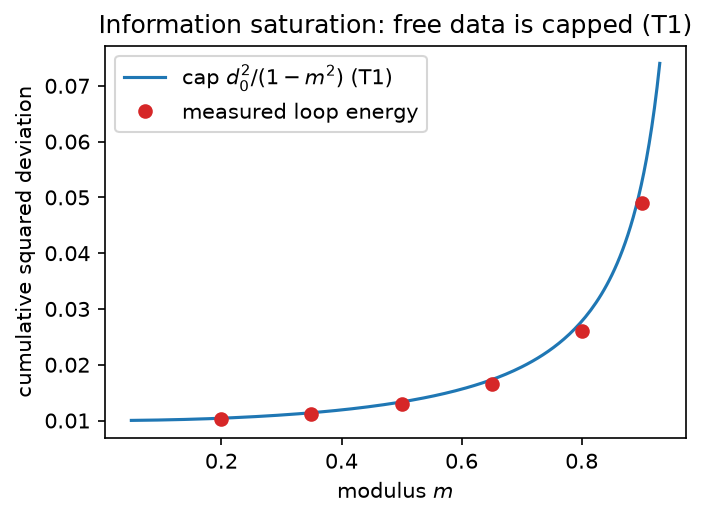
\includegraphics[width=\textwidth]{fig2_saturation.png}
\end{minipage}\hfill
\begin{minipage}{0.48\textwidth}
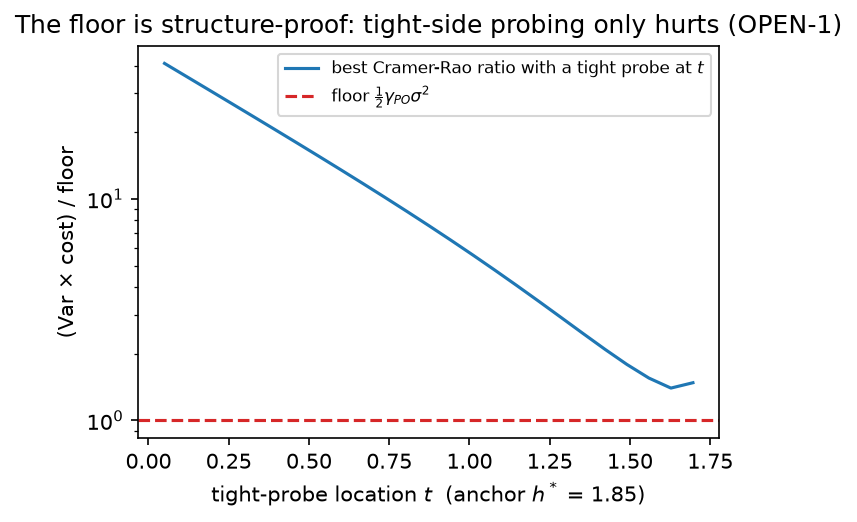
\includegraphics[width=\textwidth]{fig6_open1.png}
\end{minipage}\\[4pt]
\begin{minipage}{0.48\textwidth}
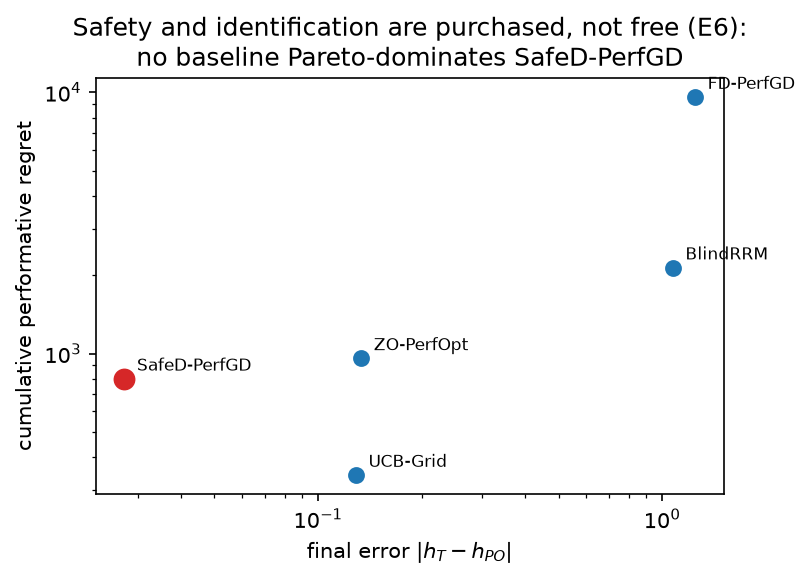
\includegraphics[width=\textwidth]{fig5_baselines.png}
\end{minipage}\hfill
\begin{minipage}{0.48\textwidth}
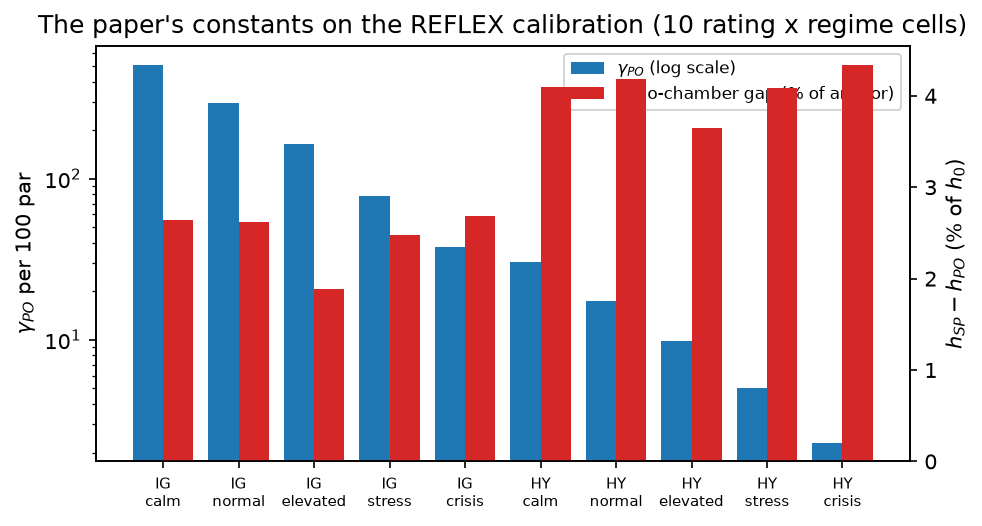
\includegraphics[width=\textwidth]{fig7_realdata.png}
\end{minipage}
\caption{\textbf{Top left:} information saturation --- measured loop energy against the cap $d_0^2/(1-m^2)$ (T1). \textbf{Top right:} the floor is structure-proof --- best Cram\'er--Rao ratio with a tight probe at $t$; tight-side probing only hurts (OPEN-1). \textbf{Bottom left:} baseline Pareto frontier --- no baseline dominates SafeD-PerfGD on (final error, regret). \textbf{Bottom right:} the paper's constants on the real-data calibration, 10 rating$\times$regime cells.}
\end{figure}

\section{Reproducibility}
\label{app:repro}

All results are deterministic from seeds, numpy-only, CPU-only. The repository contains: the derivation documents and theorem register (25 results; 34 numerical derivation checks), the pipeline (environments, estimators, designs, agents, baselines; 36 measured-vs-predicted rows; 9 unit tests), the real-data leg with its 10/10 port validation, and continuous integration running the full verification on every push. The register of ten measurement-forced pivots --- each recorded in the code where it happened, with the failed prediction and the fix --- is in the repository README.

\end{document}
